\chapter{С учетом магнитных подуровней}\label{ch:ch2}
В настоящей главе с помощью формализма матрицы плотности, поляризационных моментов и теории возмущений строится аналитическая теория нелинейных резонансов в методе ДСС с учётом реальной структуры уровней энергии в атоме, различных релаксационных процессов, движения атомов в газе и произвольных параметров поляризации лазерных пучков.
В ходе теоретического анализа в показателе поглощения среды выделены и проанализированы слагаемые, ответственные за различные линейные и нелинейные эффекты, в частности, самонасыщение среды каждым из пучков по-отдельности, насыщенное поглощение, как результат взаимодействия встречных пучков через среду резонансных атомов, а также два типа эффектов, связанных с явлением когерентного пленения населённостей (КПН) \cite{Arimondo1996,Smirnov1989}.
Каждый из пучков включает в себя две спектральные компоненты с частотами $\omega_1,\omega_2$ и волновыми векторами $k_1,k_2$.
В данной работе используется формализм поляризационных моментов. Электрическое поле имеет следующий вид:
\begin{multline} \label{eqn:field}
    \boldsymbol{E}(z,t)=\xiB_1
        \left(
            E_1e^{i(k_1z-\omega_1t)}+E_2e^{i(k_2z-\omega_2t)}
        \right)+\\+
    \xiB_2
        \left(
            E_3e^{-i(k_1z+\omega_1t+\phi_1)}+E_4e^{-i(k_2z+\omega_2t+\phi_2)}
        \right)+\\+C.C.
\end{multline}
Здесь $E_{1,2}$ и $E_{3,4}$ --- вещественные амплитуды, соответствующие волнам бегущими вдоль оси $z$ в положительном и отрицательном направлениях соответственно. Фазы $\phi_1, \phi_2$ введены для описания разности фаз между противоположно направленными пучками. 
Интенсивность лазерного поля считаем однородной вдоль сечения пучков.
Два вектора $\boldsymbol{E}_{1,2}=E_{1,2}\xiB_{1}$ имеют эллиптическую поляризацию с направлением главной оси эллипса вдоль оси $x$, в то время как главная ось векторов $\boldsymbol{E}_{3,4}=E_{3,4}\xiB_{2}$ повёрнута на уголь $\alpha$ относительно главной оси первого эллипса. 

\begin{equation} \label{eqn:xi}
    \begin{aligned}
        &\xiB_1 = -\sin{\left(\epsilon_1 - \frac{\pi}{4}\right)}\boldsymbol{a}_{-1} - \cos{\left(\epsilon_1 - \frac{\pi}{4}\right)}\boldsymbol{a}_{+1}, \\
        &\xiB_2 = -\sin{\left(\epsilon_2 - \frac{\pi}{4}\right)}e^{ - i\alpha}\boldsymbol{a}_{-1} - \cos{\left(\epsilon_2 - \frac{\pi}{4}\right)}e^{ i\alpha}\boldsymbol{a}_{+1}.
    \end{aligned}
\end{equation}
Здесь $\epsilon_{1,2}$ --- параметры эллиптичности, определённые в интервале $-\frac{\pi}{4} \leq \epsilon \leq \frac{\pi}{4}$, векторы $\boldsymbol{a}_{\pm 1}$ --- комплексные единичные векторы поляризации в сферическом базисе, соответствующие $\sigma_{\pm}$ оптическим дипольным переходам в атоме.
\begin{figure}[ht]
    \centerfloat{
        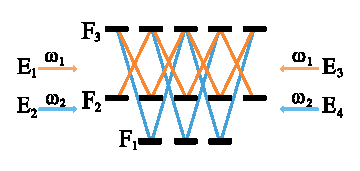
\includegraphics[width=0.65\textwidth]{levels.eps}
    }
    \caption{Пример рассматриваемых уровней энергии и индуцируемых переходов для $F_{1}=1, F_{2}=F_{3}=2$ под действием лазерного излучения.}\label{fig:latex}
\end{figure}

\FloatBarrier
